% Needle: IEEE conference paper version of the thesis (TA).
% Build: see paper/README.md  (tectonic main.tex  or  latexmk -pdf main.tex)
% Numbers: docs/thesis/chapters-id/ (newest, 2026-10-27) and logs/2026-10-13-peer-review-reanalysis.md.
% To extend to 8 pages, see the "EXTEND" comments.
\documentclass[conference]{IEEEtran}
\IEEEoverridecommandlockouts
\usepackage{cite}
\usepackage{amsmath,amssymb}
\usepackage{graphicx}
\usepackage{booktabs}
\usepackage{multirow}
\usepackage{xcolor}
\usepackage{url}
\usepackage[hidelinks]{hyperref}
\graphicspath{{figures/}}

% PLACEHOLDER: the few-shot baseline (B0-FS, issue #9) has not been run yet.
% Run `bash scripts/run_fewshot_b0.sh` on the RunPod pod, download the result folder,
% then `python -P paper/fill_fewshot.py results/<date>-b0-fewshot` overwrites this file.
\newcommand{\FSpending}{1}
\newcommand{\FSem}{\textit{pend.}}
\newcommand{\FSemdone}{\textit{pend.}}
\newcommand{\FSpgem}{\textit{pend.}}
\newcommand{\FSprec}{\textit{pend.}}
\newcommand{\FScov}{\textit{pend.}}
\newcommand{\FSdone}{\textit{pend.}}

\newcommand{\pgem}{P-gEM}

\begin{document}

\title{Rewarding the Evidence, Not Just the Answer:\\
Verifiable Evidence-Grounded Rewards for Training\\ Search Agents with GRPO}

\author{\IEEEauthorblockN{Emirsyah}
\IEEEauthorblockA{\textit{School of Computing, Telkom University}\\
Bandung, Indonesia}}

\maketitle

\begin{abstract}
Search agents trained with reinforcement learning (RL) are usually rewarded only for a correct final answer, which says nothing about whether the agent found or can show the evidence behind it. We study a judge-free alternative, VEGR (Verifiable Evidence-Grounded Reward). The agent answers with sentence-level citations, and VEGR checks every citation by rule against HotpotQA's gold supporting facts. It rewards correct answers, correct citations and useful searches, and it penalizes invalid actions. We train Qwen2.5-7B-Instruct with LoRA using a GRPO-style policy gradient on a single 48\,GB GPU; the agent searches the question's own 10 paragraphs with BM25. Sixteen runs cover five configurations with three seeds plus one diagnostic run, evaluated on a frozen 300-question holdout with seed-aware bootstrap intervals. Training lifts exact match (EM) by about 20 points over the un-tuned model (22.3\%), mostly because the agent learns the action protocol: EM on completed episodes rises only from 39.4\% to 45.2\%. Answer-only reward and the full VEGR package reach the same accuracy ($+1.0$ EM, 95\% CI $[-3.6, +5.4]$). Under answer-only reward, which penalizes an invalid citation with $-1$ but never rewards a correct one, 2 of 3 seeds stop citing. VEGR raises precision-grounded EM by 24.4 points (CI $[+8.8, +37.3]$) but does not raise evidence coverage over the un-tuned model. Grounding must be rewarded and measured explicitly; accuracy alone does not reveal it.
\end{abstract}

\begin{IEEEkeywords}
retrieval-augmented generation, search agents, reinforcement learning, verifiable rewards, citation grounding, multi-hop question answering
\end{IEEEkeywords}

\section{Introduction}

Retrieval-augmented generation lets a large language model (LLM) answer from retrieved documents rather than from memory alone. \emph{Search agents} go further: the model decides when to search, what to search for, and when to stop and answer~\cite{yao2023react}. Prompting alone does not reliably produce good search behaviour, so recent work trains search agents with RL. Search-R1~\cite{jin2025searchr1} and its successors~\cite{song2025r1searcher,chen2025research,zheng2025deepresearcher} use an \emph{outcome reward}: the episode scores 1 if the final answer matches the gold answer. GRPO~\cite{shao2024deepseekmath,deepseek2025r1} made this cheap by replacing the learned critic with a group-relative baseline.

An outcome reward is a proxy. A correct answer does not show that the agent found, used, or can point to the evidence behind it, and optimizing a proxy invites behaviour that scores well without doing what was intended~\cite{skalse2022reward,gao2023overoptimization}. Citation-aware rewards exist~\cite{zhang2026carr,huang2024citations}, but they typically rely on an LLM judge or a trained model, which adds an extra model to the training loop and its own biases. Most RL results for search agents are also reported from single runs, although seed variance in RL is large~\cite{henderson2018matters,agarwal2021precipice}.

HotpotQA~\cite{yang2018hotpotqa} offers a cheap way to study this. Its questions are annotated with the exact sentences that support the answer, so a sentence-level citation can be checked by rule, without a judge. We use this to ask three questions:
\begin{itemize}
\item \textbf{RQ1:} Does GRPO-style training improve a 7B search agent over the un-tuned model?
\item \textbf{RQ2:} Does a verifiable evidence-grounded reward prevent the shortcut behaviour of answer-only reward, without losing accuracy?
\item \textbf{RQ3} (exploratory): How do reward variants and optimizer changes affect grounding and search behaviour?
\end{itemize}

Our contributions are: (i) VEGR, a judge-free, sentence-level, protocol-enforcing reward for multi-turn search agents; (ii) evidence, from three seeds and the training rollouts, that answer-only reward drops citations on two of three seeds, with a mechanism traced in the training rollouts; (iii) a controlled comparison with seed-aware bootstrap intervals that separates reward changes from optimizer changes; and (iv) an open single-GPU pipeline that trains and evaluates one configuration in about two GPU-hours. We do not propose a new RL algorithm, we do not claim state-of-the-art accuracy, and the individual reward terms are not new; the contribution is their combination and the controlled evidence about what it changes.

\section{Related Work}

\textbf{RL for search agents.} Search-R1~\cite{jin2025searchr1}, R1-Searcher~\cite{song2025r1searcher}, ReSearch~\cite{chen2025research} and DeepResearcher~\cite{zheng2025deepresearcher} train LLMs to interleave reasoning with search calls using outcome rewards. AutoRefine~\cite{shi2025autorefine} adds a retrieval-specific reward, and StepSearch~\cite{wang2025stepsearch}, PROGRESS~\cite{paul2026progress} and dense process supervision~\cite{zhu2026dense,huang2026retrievalcredit} assign credit to individual search steps. STAMP~\cite{xu2026stamp} uses provenance to assign credit to search turns. These works mostly report multi-GPU training on open corpora and score the final answer, not its citations.

\textbf{Evidence and citation rewards.} ALCE~\cite{gao2023alce} separates citation precision from citation recall and shows that models are often precise but incomplete. Fine-grained RLHF~\cite{wu2023finegrained} and Huang et al.~\cite{huang2024citations} reward citations with learned or NLI-based scorers. CaRR~\cite{zhang2026carr} trains deep-search agents with citation-aware rubric rewards scored by an LLM judge and reports that outcome-only GRPO learns shortcut answers. VEGR is a small-scale, judge-free counterpart: its evidence terms are exact set comparisons against gold labels, so they need no extra model and are deterministic and reproducible, but they require gold supporting facts.

\textbf{GRPO and its variants.} GRPO~\cite{shao2024deepseekmath} normalizes each reward within a group of rollouts of the same prompt. Dr.\ GRPO~\cite{liu2025drgrpo} shows that the standard-deviation and length normalizations bias the update; DAPO~\cite{yu2025dapo} adds dynamic sampling, which skips zero-variance groups. We test one change from each (Sec.~\ref{sec:setup}).

\section{Method}
\label{sec:method}

\begin{figure*}[t]
\centering
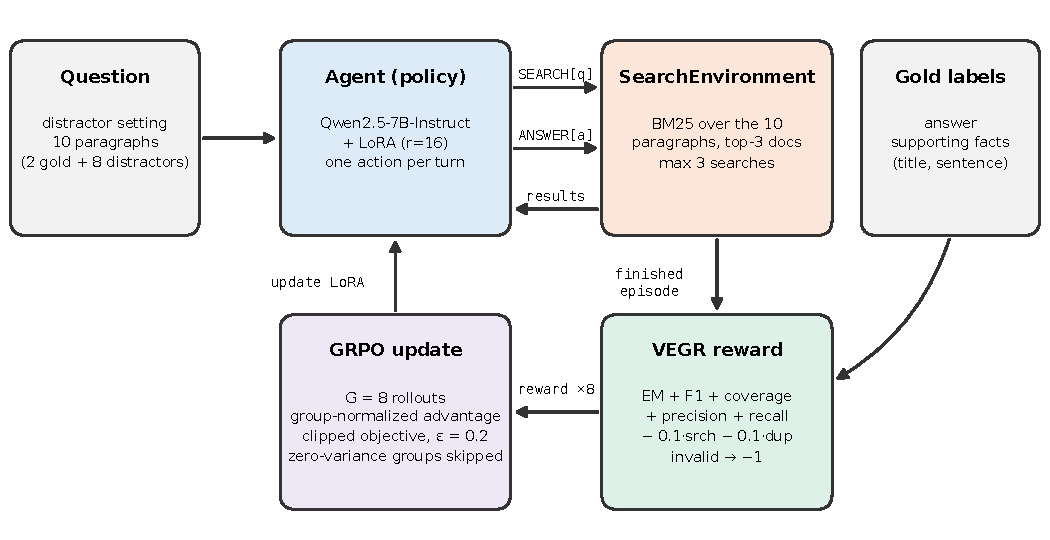
\includegraphics[width=0.86\textwidth]{fig3_1_system.pdf}
\caption{One training step. The agent receives a HotpotQA question, issues up to three \texttt{SEARCH} actions over the question's 10 paragraphs, and ends with \texttt{ANSWER[a] CITATIONS[title|index; \ldots]}. VEGR scores the finished episode against the gold answer and supporting facts; GRPO compares the rewards of 8 episodes of the same question and updates the LoRA adapter.}
\label{fig:system}
\end{figure*}

\subsection{Environment and Action Protocol}
Each episode is one HotpotQA question in the distractor setting: 10 Wikipedia paragraphs, 2 gold and 8 distractors, with gold supporting facts given as (title, sentence index) pairs. The searchable corpus is the question's own 10 paragraphs, indexed with Okapi BM25~\cite{robertson2009bm25}; each search returns the top 3 whole paragraphs with numbered sentences, and an episode allows at most 3 searches. This closed corpus makes retrieval easy (the un-tuned model already reaches retrieval recall 0.83), so the task is closer to reading comprehension with a page-finding tool than to web search. Each turn the agent emits exactly one action (Fig.~\ref{fig:system}): \texttt{SEARCH[query]}, or the terminal \texttt{ANSWER[answer] CITATIONS[title|index; \ldots]}.

An episode is \emph{invalid} on a \emph{protocol failure} (output not in the grammar), an \emph{evidence failure} (a citation to a title that is not one of the question's 10 paragraphs, an out-of-range sentence index, or a duplicate citation; mostly invented or mis-copied titles), or a \emph{search-limit failure} (no answer after the last search). An answer with an empty citation list is valid; we keep this loophole so that all runs share one environment.

\subsection{VEGR}
Let $G$ be the gold supporting facts and $C$ the cited sentences. For a valid episode,
\begin{equation}
R = \mathrm{EM} + \mathrm{F1} + \mathrm{Cov} + \mathrm{Prec} + \mathrm{RetR} - 0.1\,\mathrm{Srch} - 0.1\,\mathrm{Dup},
\label{eq:vegr}
\end{equation}
where EM and F1 compare the normalized answer with the gold answer, $\mathrm{Cov}=|G\cap C|/|G|$ is evidence coverage, $\mathrm{Prec}=|G\cap C|/|C|$ is citation precision (0 when $C$ is empty), RetR is the fraction of gold paragraphs returned by any search, Srch is searches used over the search limit, and Dup is the fraction of repeated queries. An invalid episode receives $R=-1$. The weights are untuned defaults. For example, two correct answers to the same question score 4.93 (both gold sentences cited, both gold paragraphs retrieved) and 2.47 (no citation, one paragraph retrieved) under VEGR, but 1 and 1 under answer-only reward.

\textbf{Reward variants.} \textbf{R0} (outcome-only) is $R=\mathrm{EM}$, still with $-1$ for invalid episodes; it mirrors Search-R1. \textbf{R1} is full VEGR. \textbf{R2} applies the search and duplicate penalties only when EM\,=\,1. \textbf{R3} doubles the coverage weight.

Note what R0 does to citations: it never rewards a correct citation, but an invalid one turns the episode into a $-1$ evidence failure. Citing helps only indirectly, if cited answers are more often correct, so whether it pays off depends on how often the policy's citations are invalid.

\subsection{Policy and Training}
The policy is Qwen2.5-7B-Instruct~\cite{qwen2024qwen25} in bf16 with a LoRA adapter~\cite{hu2022lora} ($r=16$, $\alpha=32$) on all attention and MLP projections. The prompt states the action grammar with one example, the question, the number of searches left and all search results so far, and is rebuilt every turn.

For each training question the current policy samples $G=8$ full episodes (temperature 1.0). Rewards are normalized within the group, $A_i=(r_i-\bar r)/(\mathrm{std}(r)+10^{-6})$, and every action in an episode shares its advantage. Groups in which all 8 rewards are equal carry no signal and are skipped. The loss is the PPO-style clipped surrogate~\cite{schulman2017ppo} ($\epsilon=0.2$) on the sequence-mean log-probability of the agent's tokens, with no KL term. Because each group is used for exactly one optimizer step, the old and new policies coincide at the update and clipping never fires (the logged clip fraction is 0 in all 16 runs): in practice the update is REINFORCE with a group-mean baseline and group-normalized advantages. Each run makes one pass over 256 training questions (AdamW, learning rate $2\times10^{-5}$).

\textbf{Optimizer variants.} \textbf{R4} uses VEGR with $A_i=r_i-\bar r$ (no standard-deviation division). This is one of the two Dr.\ GRPO changes~\cite{liu2025drgrpo}, not full Dr.\ GRPO: the sequence-level length normalization is kept. \textbf{R0-dyn} is R0 with DAPO-style dynamic sampling~\cite{yu2025dapo}: zero-variance groups do not count, and the trainer draws up to 512 questions until it has made 256 real updates.

\section{Experimental Setup}
\label{sec:setup}

\textbf{Data.} HotpotQA v1.1 train is split by a deterministic hash into 85{,}573 training and 4{,}452 validation questions. The holdout is a frozen set of 300 dev questions that was never used to choose settings. Each run samples 256 training questions with its seed.

\textbf{Runs.} B0 is the un-tuned model. R0--R4 are each trained with seeds 7, 8 and 9; R0-dyn uses seed 8 only, the seed on which R0 collapsed. The seed fixes both the training sample and the sampling noise. B0, R0, R1 and R2 were planned before the multi-seed batch; R3, R4 and R0-dyn were added after the R0--R2 holdout results were known, so we treat them as exploratory. \textbf{B0-FS} is a prompt-only control: the un-tuned model with one fictional two-hop worked example prepended to the prompt (issue \#9)\ifnum\FSpending=1{}; \textcolor{red}{its run is pending (Sec.~\ref{sec:discussion})}\fi.

\textbf{Evaluation.} All models are evaluated on the same 300 holdout questions with greedy decoding and no retries. \emph{EM (all)} counts invalid episodes as 0. \emph{Precision-grounded EM} (\pgem) counts an episode only if EM\,=\,1, it has at least one citation, and every citation is a gold fact; it is strict on wrong citations but lenient on missing ones, so we also report HotpotQA's \emph{Sup-EM} (cited set equals gold set) and \emph{Joint-EM} (EM and Sup-EM). Precision and coverage are averaged over completed episodes.

\textbf{Statistics.} The primary intervals are a seed-aware paired bootstrap: each of 10{,}000 resamples draws 3 seeds with replacement per method and 300 questions with replacement, shared across methods; we report the 95\% percentile interval. Primary comparisons are RQ1 (every method vs.\ B0) and R1$-$R0; the rest are exploratory and uncorrected for multiple comparisons, and a non-significant exploratory difference is read as inconclusive.

\textbf{Compute.} All runs use a single NVIDIA L40S GPU (48\,GB); one run (training plus holdout evaluation) takes about 2.05\,h of wall-clock time. Software: Transformers 4.57.6, PEFT 0.21.2; PyTorch 2.14.1 for B0 and R1 seed 7 and 2.11.0 for later runs because of a driver change.

\section{Results}
\label{sec:results}

\begin{table*}[t]
\centering
\caption{Holdout results: mean $\pm$ s.d.\ over seeds 7, 8, 9 (B0, B0-FS and R0-dyn: one evaluation). EM, completed-only EM, \pgem, Sup-EM and Joint-EM in \%; precision and coverage averaged over completed episodes.}
\label{tab:main}
\footnotesize\setlength{\tabcolsep}{3.5pt}
\begin{tabular}{lcccccccc}
\toprule
Method & EM & EM (completed) & \pgem & Sup-EM & Joint-EM & Cit.\ precision & Evid.\ coverage & Completed /300 \\
\midrule
B0 un-tuned & 22.3 & 39.4 & 13.0 & 11.3 & 6.0 & 0.633 & 0.472 & 170 \\
B0-FS few-shot prompt & \FSem & \FSemdone & \FSpgem & -- & -- & \FSprec & \FScov & \FSdone \\
\midrule
R0 outcome-only & 42.6$\pm$2.2 & 43.8$\pm$2.6 & 8.2$\pm$14.2 & 5.0$\pm$8.7 & 3.2$\pm$5.6 & 0.207$\pm$0.358 & 0.146$\pm$0.253 & 278--299 \\
\textbf{R1 VEGR} & 43.6$\pm$1.5 & 45.2$\pm$1.0 & \textbf{32.7$\pm$4.8} & 11.9$\pm$10.1 & 7.1$\pm$5.8 & \textbf{0.744$\pm$0.015} & 0.440$\pm$0.095 & 287--293 \\
R2 gated penalties & 42.7$\pm$5.4 & 44.7$\pm$5.2 & 29.8$\pm$3.1 & 15.9$\pm$4.8 & 10.0$\pm$1.9 & 0.718$\pm$0.026 & 0.483$\pm$0.051 & 283--290 \\
R3 coverage $\times$2 & 42.3$\pm$2.0 & 44.6$\pm$2.6 & 24.7$\pm$5.4 & \textbf{24.3$\pm$4.2} & \textbf{13.4$\pm$2.2} & 0.690$\pm$0.053 & \textbf{0.569$\pm$0.033} & 282--289 \\
R4 no std norm. & 44.0$\pm$4.0 & 45.3$\pm$3.8 & 31.0$\pm$7.7 & 12.4$\pm$8.7 & 7.4$\pm$5.3 & 0.695$\pm$0.060 & 0.441$\pm$0.085 & 288--293 \\
R0-dyn (seed 8) & 48.7 & 48.7 & 0.0 & 0.0 & 0.0 & 0.000 & 0.000 & 300 \\
\bottomrule
\end{tabular}
\end{table*}

\begin{table}[t]
\centering
\caption{Paired differences in points with seed-aware 95\% bootstrap intervals (10{,}000 resamples). Rows below the line are exploratory.}
\label{tab:ci}
\setlength{\tabcolsep}{2.5pt}
\resizebox{\columnwidth}{!}{%
\begin{tabular}{lccc}
\toprule
Comparison & $\Delta$EM & $\Delta$\pgem & $\Delta$Joint-EM \\
\midrule
R0$-$B0 & $+20.2\,[+15.1,+25.6]$ & $-4.8\,[-16.0,+10.7]$ & $-2.8\,[-8.0,+3.4]$ \\
R1$-$B0 & $+21.2\,[+16.4,+26.0]$ & $+19.7\,[+13.3,+26.1]$ & $+1.1\,[-5.1,+6.9]$ \\
\textbf{R1$-$R0} & $+1.0\,[-3.6,+5.4]$ & $\mathbf{+24.4\,[+8.8,+37.3]}$ & $+3.9\,[-4.0,+11.4]$ \\
\midrule
R2$-$R1 & $-0.9\,[-7.1,+5.8]$ & $-2.9\,[-9.8,+3.6]$ & $+2.9\,[-2.9,+9.3]$ \\
R3$-$R1 & $-1.2\,[-5.7,+3.3]$ & $-8.0\,[-16.1,-0.2]$ & $+6.3\,[+0.2,+13.1]$ \\
R4$-$R1 & $+0.4\,[-5.2,+5.7]$ & $-1.7\,[-10.9,+7.7]$ & $+0.3\,[-7.0,+8.1]$ \\
\bottomrule
\end{tabular}}
\end{table}

\subsection{RQ1: Training vs.\ the Un-tuned Model}
The un-tuned model reaches 22.3\% EM, but mainly because only 170 of 300 episodes complete: of its 130 failures, 85 are evidence failures (mostly invented titles), 37 protocol failures and 8 search-limit failures. Every trained method gains about 20 EM points, and every seed-aware interval excludes zero (Table~\ref{tab:ci}; R2$-$B0, R3$-$B0 and R4$-$B0 are $+20.3$, $+20.0$ and $+21.7$). Most of this is protocol learning, not better answers: no trained run loses more than 22 episodes, while EM on completed episodes moves only from 39.4\% to 43.8--45.3\% (Table~\ref{tab:main}). In R1 seed 7 the invalid-rollout rate falls from 46\% to 7\% over the first five 32-step blocks. \ifnum\FSpending=1 Whether prompting alone recovers part of this protocol gain is tested by B0-FS, whose run is pending.\else With one worked example in the prompt, the un-tuned model reaches \FSem\% EM (\FSdone/300 completed), which bounds how much of the gain prompting alone recovers.\fi

\subsection{RQ2: Outcome-Only Reward vs.\ VEGR}
\textbf{Same accuracy.} R1$-$R0 is $+1.0$ EM with interval $[-3.6,+5.4]$; no accuracy difference can be claimed.

\textbf{Very different grounding.} VEGR raises \pgem{} by 24.4 points over R0 (seed-aware interval $[+8.8,+37.3]$), the largest between-method effect in the study (Fig.~\ref{fig:emprec}). The interval is wide because R0's grounding varies so much across seeds (24.7\%, 0\%, 0\%). Two R0 seeds (8 and 9) learn to answer with \emph{no citations at all}: all 122 and 135 of their correct answers are uncited, so their precision, coverage and \pgem{} are 0. Seed 9 still searches 2.27 times per episode and retrieves the gold paragraphs (recall 0.86), then does not cite them. R0 seed 7 keeps citing at B0-level precision (0.621) but always uses all three searches, and 229 of its 278 completed episodes repeat a query, a reward-neutral drift since R0 gives the search penalty zero weight. With three seeds, the 95\% Clopper--Pearson interval for the collapse rate (2 of 3) is $[0.09, 0.99]$. R1 is the most stable method: EM 42.7--45.3\% and precision 0.726--0.754 on all seeds. The precision gain is not a selection effect: on the 136 questions completed by every run, precision is 0.627 for B0, 0.646 for R0 seed 7 and 0.750--0.790 for R1.

Note that R1 and R0 differ in six reward terms and in the number of updates (about 240 vs.\ 130), so this comparison measures the whole VEGR package and the training signal it creates, not one term.

\begin{figure}[t]
\centering
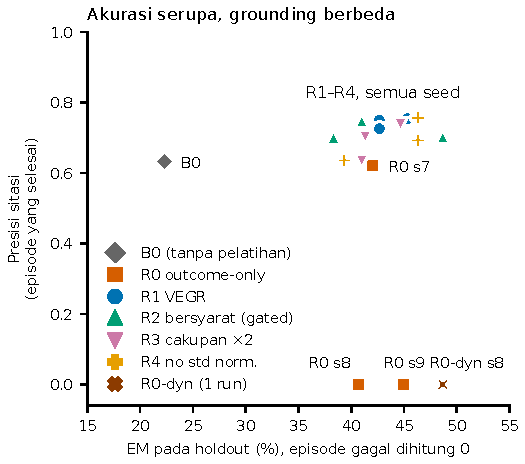
\includegraphics[width=\columnwidth]{fig4_3_em_vs_precision.pdf}
\caption{Holdout EM (failures count as 0) against citation precision (completed episodes), one point per run. All trained runs share one accuracy band; only the evidence-rewarded runs keep citing.}
\label{fig:emprec}
\end{figure}

\textbf{Why R0 stops citing.} The training rollouts explain seed 8. In the first 32 steps of R0 seed 8, 176 rollouts tried to cite: 90 were evidence failures ($-1$) and 86 were valid with mean reward 0.50, while 42 uncited valid rollouts averaged 0.36. A valid citation was worth slightly more, because cited answers were more often correct, but the expected reward of \emph{trying} to cite was $(86\times0.50-90)/176\approx-0.27$ against $+0.36$ for not citing. Seed 9 is only partly explained: fewer of its early citation attempts were invalid (23\% vs.\ 51\%), so trying to cite was not a losing bet in its first block ($+0.29$ vs.\ $+0.26$), yet it too stopped citing from step 97 on. Seed 7 kept citing with a 36\% early failure rate. The $-1$ penalty thus makes citing risky without making its collapse inevitable. R1 starts with the same failure rate (91 evidence failures in its first block), but under VEGR a valid cited rollout earns about 3.4 against 1.3 uncited, and valid cited rollouts grow from 85 to 214 per block. In short, R0 penalizes bad citations but never rewards good ones; VEGR rewards correct ones. (Rollout logs store no citation lists, so ``tried to cite'' counts evidence failures plus valid rollouts with a gold citation.)

\textbf{Zero-variance groups.} R0's binary reward also starves GRPO of signal: R0 skips 107, 128 and 124 of 256 steps, against 8--20 for the evidence-rewarded runs, whose continuous terms almost always separate the 8 rollouts (Fig.~\ref{fig:skipped}).

\begin{figure}[t]
\centering
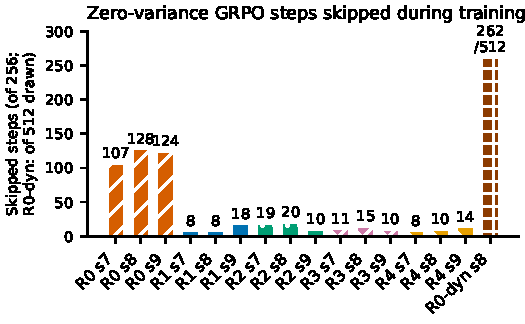
\includegraphics[width=\columnwidth]{fig4_1_skipped_steps.pdf}
\caption{Training steps skipped because all 8 rollouts of the group received the same reward (of 256; R0-dyn: of 512 questions drawn).}
\label{fig:skipped}
\end{figure}

\textbf{Precise but incomplete.} VEGR makes citations correct, not complete. R1's coverage (0.440) is no higher than B0's (0.472): the policy prefers a few early sentences (93\% of R1 seed 8's 485 citations point to one of a paragraph's first three sentences), and under the summed reward one safe citation already earns full precision and partial coverage. R1 seed 9 has the best \pgem{} of the R1 runs (37.7\%) but cites only 1.03 sentences per episode and has Sup-EM 0.7\%, so \pgem{} must be read with Sup-EM and Joint-EM.

\subsection{RQ3: Reward and Optimizer Variants (Exploratory)}
\textbf{R2} (gated penalties) looked better on seed 8 alone (48.7\% vs.\ 42.7\%), but this did not replicate (seed 9: 38.3\% vs.\ 45.3\%); over three seeds it is inconclusive and has the widest seed spread (s.d.\ 5.4). \textbf{R3} (coverage $\times$2) reaches the highest coverage (0.569) by citing more sentences, some of them wrong: \pgem{} drops by 8.0 points vs.\ R1 (interval $[-16.1,-0.2]$), yet R3 is best on HotpotQA's own Sup-EM (24.3\%) and Joint-EM (13.4\%, $+6.3$ $[+0.2,+13.1]$). Which reward wins depends on whether the metric punishes wrong citations or requires complete evidence; both intervals sit close to zero. \textbf{R4} (no standard-deviation division) is indistinguishable from R1. \textbf{R0-dyn} reaches the highest EM of any run (48.7\%, $+8.0$ over R0 seed 8 with a question-only interval $[+3.3,+12.7]$) and completes all 300 episodes, but it drew 512 questions and made 250 updates versus 128, so the gain mixes dynamic sampling with twice the data. It still cites nothing (\pgem{} 0.0\%; all 146 correct answers uncited) and collapses on the same schedule as R0 seed 8. On the one seed tested, an optimizer fix improved accuracy but did not restore grounding.

\section{Discussion}
\label{sec:discussion}

\textbf{What the results support.} GRPO-style training with LoRA on one GPU lifts a 7B closed-corpus search agent by about 20 EM points, mostly by teaching it a valid, verifiable action protocol. Outcome-only reward and full VEGR reach statistically indistinguishable accuracy, but VEGR's precision-grounded EM is 24.4 points higher, and outcome-only reward dropped citations on two of three seeds; its definition, which punishes invalid citations and never rewards valid ones, makes this possible. This matches CaRR's report of outcome-only shortcuts~\cite{zhang2026carr} at a far smaller scale, and here it can be traced and detected by rule. It also agrees with Search-R1~\cite{jin2025searchr1} that outcome RL improves accuracy, and adds that accuracy hides whether answers are grounded.

\textbf{What they do not support.} That VEGR is more \emph{accurate}; that any single VEGR term, rather than the package, drives the grounding gain; that R2 or R4 help or hurt; that dynamic sampling can never prevent the shortcut (one seed); or that VEGR improves evidence coverage.

\textbf{Threats to validity.} Three seeds and 300 holdout questions cannot resolve EM differences of a few points. VEGR rewards precision and coverage against the same gold facts used by the grounding metrics, so part of the \pgem{} gain is a gain on the training target (Goodhart), and HotpotQA's supporting facts are known to be incomplete; an attribution check that does not use gold labels was not run. The corpus is the question's own 10 paragraphs, far easier than open-web search. Each run stops after a fixed 256 training questions, before reward has converged. PyTorch changed between B0/R1 seed 7 and later runs. The environment accepts uncited answers, which is what lets R0 collapse; it also checks cited titles against the question's 10 paragraphs rather than against search results (at least 4 holdout episodes cite a gold sentence that was never retrieved); and the citation separator collides with ``\&'' in a few titles (at most 1.7 EM points per run, similar across R1--R4). Reward weights were not tuned, and R3, R4 and R0-dyn were designed after seeing holdout results. Because RQ1's gain is mostly protocol learning, a prompt-only baseline matters: \ifnum\FSpending=1 B0-FS (one worked example in the prompt) is prepared and runs with one command (\texttt{scripts/run\_fewshot\_b0.sh}) but has not been run yet, so its row in Table~\ref{tab:main} is pending.\else B0-FS reaches \FSem\% EM and \FSpgem\% \pgem{} (Table~\ref{tab:main}).\fi

% EXTEND (8 pages): add the per-seed figure fig4_4_em_per_seed.pdf, the training-rollout
% table (chapters-id Table 4.4), Fig. 4.2 (citation precision during training) and
% two traces from chapters-id Sec. 4.7.

\section{Conclusion}
Rewarding only the answer is enough to make a small search agent more accurate, but not to make it grounded: with outcome-only reward, a citation could only lower the policy's reward, and two of three seeds stopped citing. A judge-free reward that checks sentence-level citations against gold supporting facts keeps accuracy, keeps citations precise on every seed, and needs no extra model to compute, though it does not make citations complete. Future work includes step-level credit for searches~\cite{xu2026stamp,wang2025stepsearch}, coverage-aware weighting, open-corpus retrieval, and datasets beyond HotpotQA. Code, configurations, split manifests and all episode logs are released with the project.

\bibliographystyle{IEEEtran}
\bibliography{refs}

\end{document}
